% Open participation in analysis, not permission to perform implant procedures.
\begin{frame}{OpenScope: access to an observatory, not just a dataset}
  \begin{columns}[c,onlytextwidth]
    \column{.54\textwidth}
      \small
      \NTXPoint{Allen Institute's shared platform}{External researchers propose experiments using mouse Neuropixels recordings and two-photon imaging.}
      \NTXPoint{A 2026 release to work with}{Predictive Processing data: public S3 assets and partial NWB files; complete DANDI releases follow as finalized.}
      \NTXPoint{An entry point without your own implant lab}{Use the OpenScope Databook to analyze recordings and ask new questions.}
    \column{.42\textwidth}
      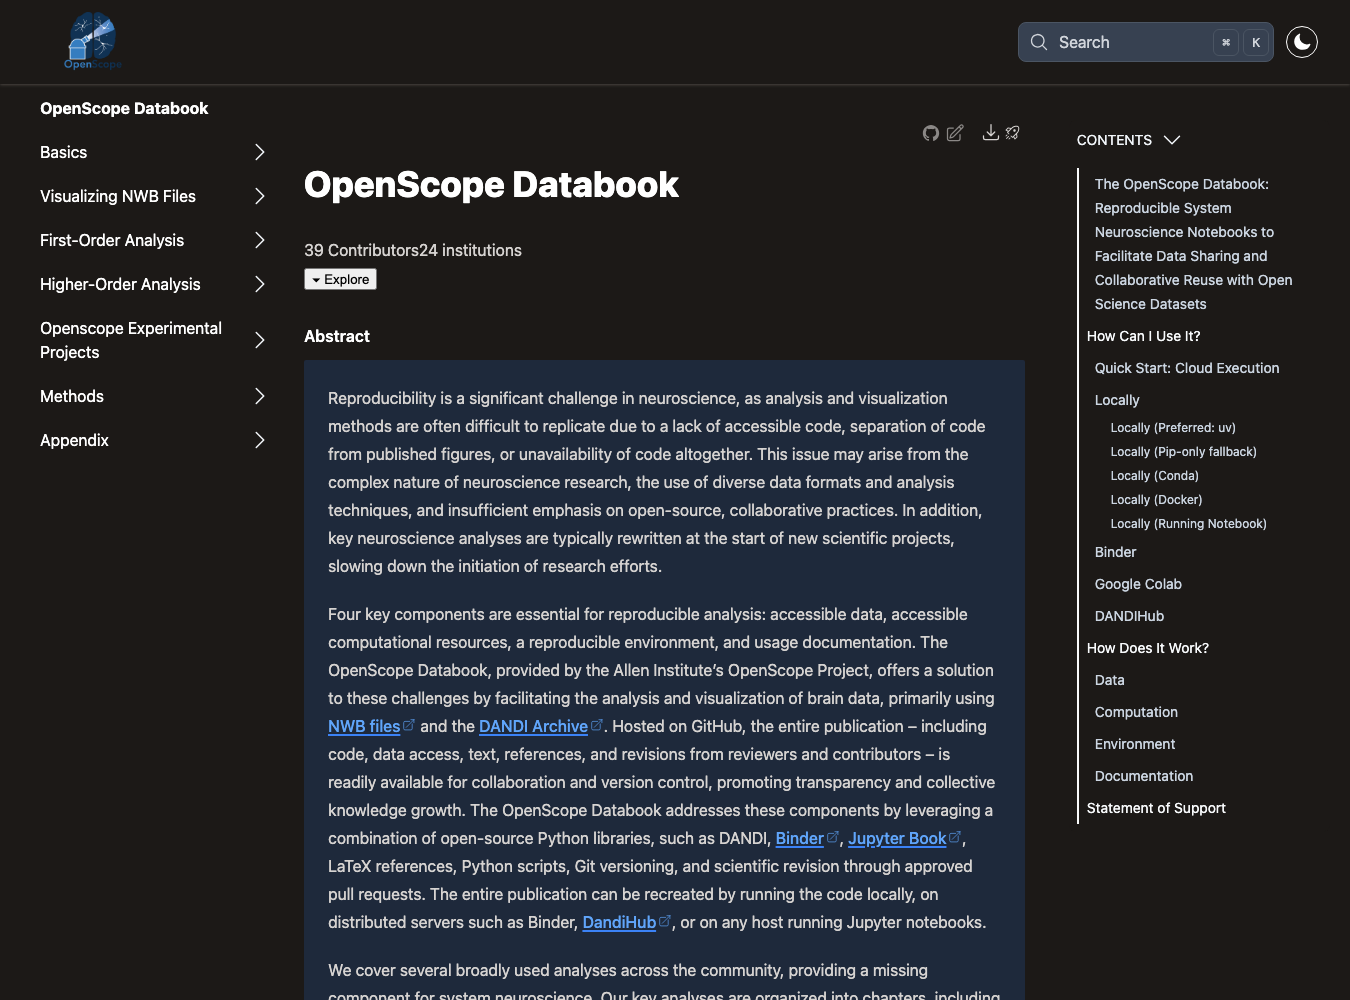
\includegraphics[width=\linewidth,height=43mm,keepaspectratio]{assets/history/openscope-databook-page.png}\par\smallskip
      {\tiny OpenScope Databook / Allen Institute\par}
  \end{columns}
  {\tiny\color{NTXMuted}Sources: \href{https://www.allenneuraldynamics.org/projects/openscope}{OpenScope}; \href{https://allenneuraldynamics.github.io/openscope-community-predictive-processing/data-access/}{2026 release guide}; \href{https://alleninstitute.github.io/openscope_databook/}{Databook}\par}
  \note{[61:15--62:45] OpenScope lowers the cost of experimental access through a selected-proposal model and makes recorded data reusable. It is primarily mouse systems neuroscience, not a human implant trial. Do not imply an application call is currently open: the program page notes no 2025 call and points to its community project. Its traditional release policy includes an embargo. The Predictive Processing guide specifically labels its release ongoing as of April 2026; complete multimodal NWB files on DANDI were still being finalized. Public S3 access needs no AWS account. We distinguish released assets from promised future completion. Reanalysis offers a way into invasive-recording methods without performing surgery or owning a recording facility.}
\end{frame}

\begin{frame}{DANDI + NWB: make invasive recordings reusable}
  \begin{columns}[c,onlytextwidth]
    \column{.53\textwidth}
      \small
      \NTXPoint{NWB is the shared data standard}{Recordings, experimental context, and metadata in a form supported by common tools.}
      \NTXPoint{DANDI is the archive}{Find datasets, inspect metadata, download or stream data, and cite the version used.}
      \NTXPoint{Access to analysis across laboratories}{Study neural signals and behavior without collecting every dataset yourself. Respect each dataset's terms.}
    \column{.43\textwidth}
      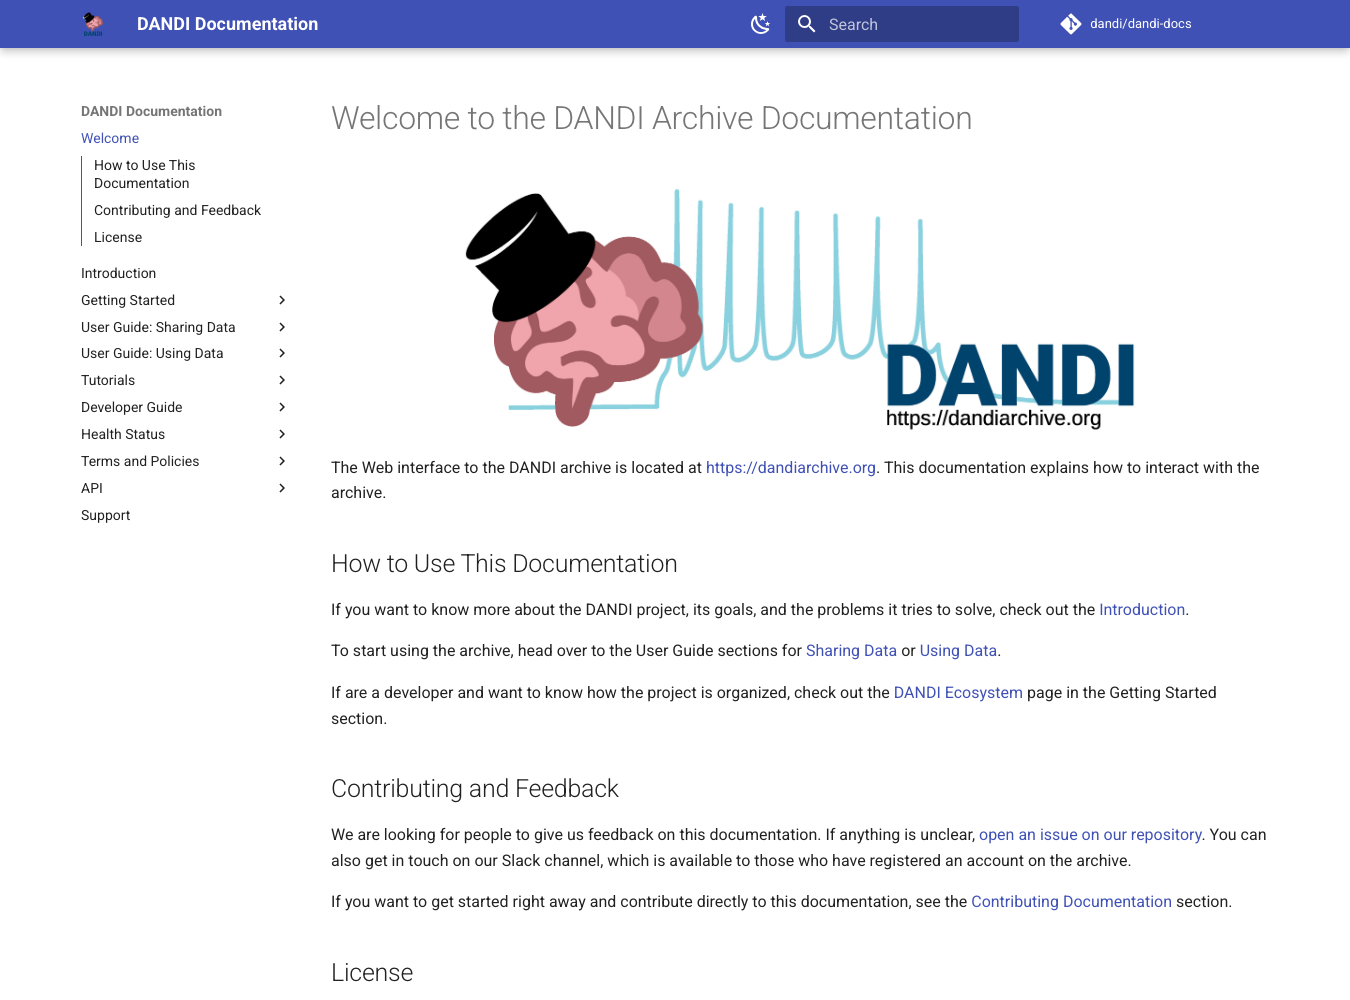
\includegraphics[width=\linewidth,height=43mm,keepaspectratio]{assets/history/dandi-documentation-page.png}\par\smallskip
      {\tiny Official DANDI archive documentation\par}
  \end{columns}
  {\tiny\color{NTXMuted}Sources: \href{https://docs.dandiarchive.org/}{DANDI documentation}; \href{https://nwb.org/}{Neurodata Without Borders}\par}
  \note{[62:45--64:15] Keep the roles clear: NWB is a neurophysiology data standard; DANDI provides discovery, storage, access and publication infrastructure. Neither is itself an implant or a clinical trial. The archive spans species and recording modalities, not exclusively human invasive BCI. Practical accessibility means fewer custom file readers, documented experimental context, and reusable analysis workflows. Streaming can reduce the need for full local downloads but does not eliminate bandwidth, compute or expertise requirements. Cite the precise Dandiset version and check its license and conditions; metadata availability does not mean all studies have identical access rules.}
\end{frame}

\begin{frame}{NeuroDataReHack 2026: learn by reusing real recordings}
  \begin{columns}[c,onlytextwidth]
    \column{.54\textwidth}
      \small
      \NTXPoint{July 12--17, HHMI Janelia}{A week of collaborative reanalysis in Ashburn, Virginia.}
      \NTXPoint{NWB + DANDI, with expert support}{OpenScope data, spike analysis, visualization, and independent projects; recorded talks are public.}
      \NTXPoint{Lower the participation barrier}{No registration fee; lodging and meals provided for participants. Travel remained their responsibility.}
    \column{.42\textwidth}
      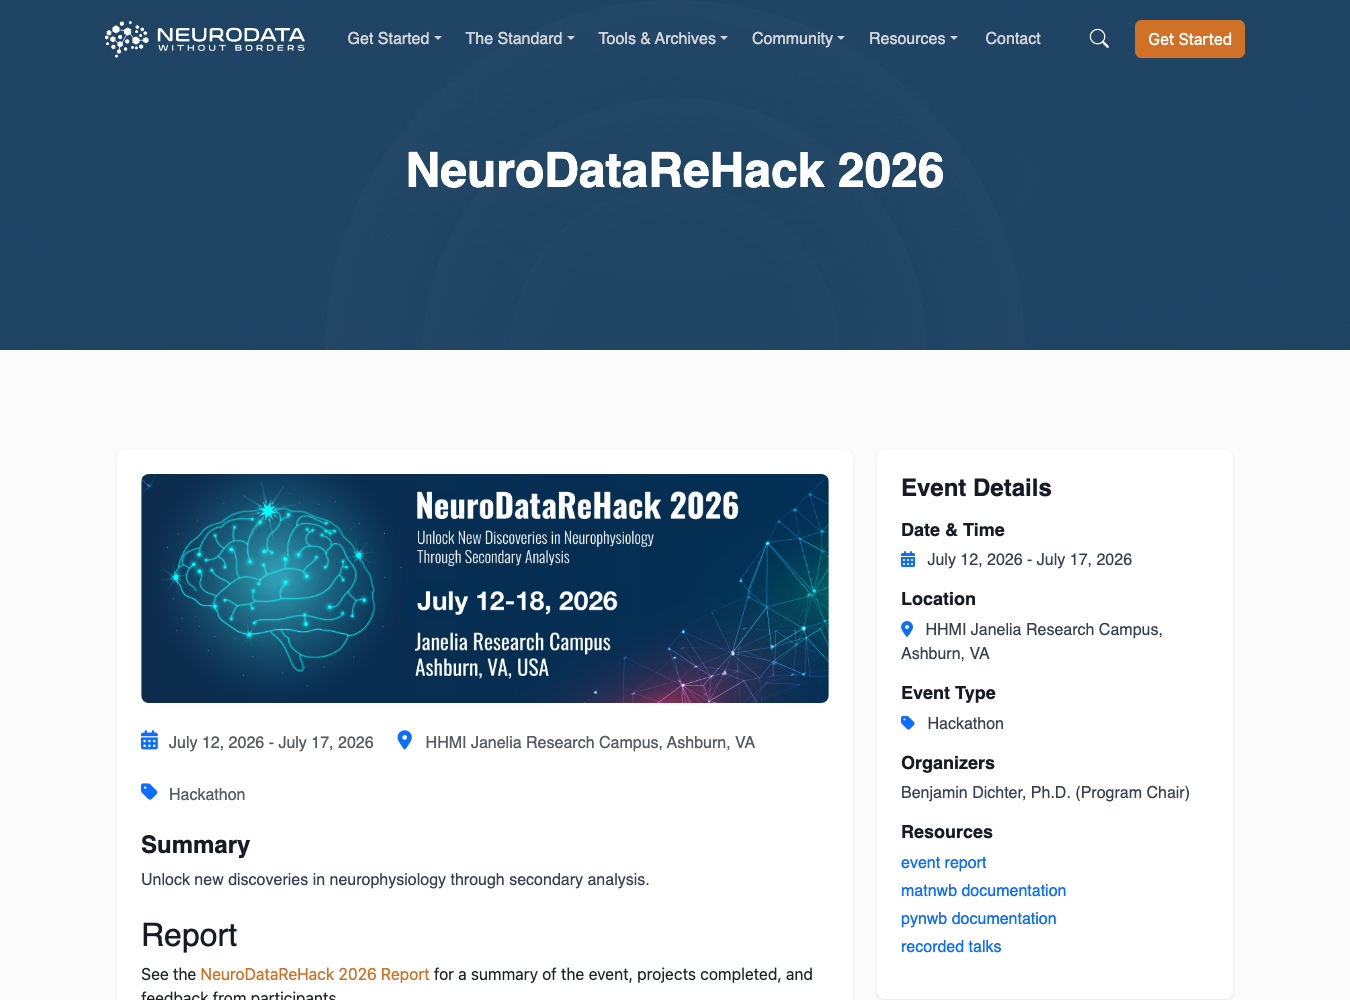
\includegraphics[width=\linewidth,height=43mm,keepaspectratio]{assets/history/neurodatarehack-2026-page.png}\par\smallskip
      {\tiny Official 2026 event page / NWB\par}
  \end{columns}
  \NTXSource{https://nwb.org/events/hck26-2026-janelia-ndrh/}{NeuroDataReHack 2026: program, report, and recordings}
  \note{[64:15--65:45] This summer's event has already happened; do not present registration as open. Its focus was secondary analysis rather than converting new data to NWB. Admission was selective and basic programming plus neurophysiology experience were expected, so free attendance does not mean unrestricted admission. Recorded teaching extends access beyond the cohort. These resources help people contribute computational work on invasive recordings while original data collection remains with qualified laboratories. No NTX organizing role is asserted.}
\end{frame}

\begin{frame}{Neuro Galaxy: from open recordings to shared models}
  \begin{columns}[c,onlytextwidth]
    \column{.54\textwidth}
      \small
      \NTXPoint{Tools for neural foundation models}{\texttt{torch\_brain}: data loading, training pipelines, and models across recordings.}
      \NTXPoint{Hands-on learning at Janelia ReHack}{Alexandre Andre's \emph{Applying Neural Foundation Models} tutorial used \texttt{torch\_brain}.}
      \NTXPoint{A project our community can take on}{Start with public recordings, reproduce a decoder, then test transfer across sessions or subjects.}
    \column{.42\textwidth}
      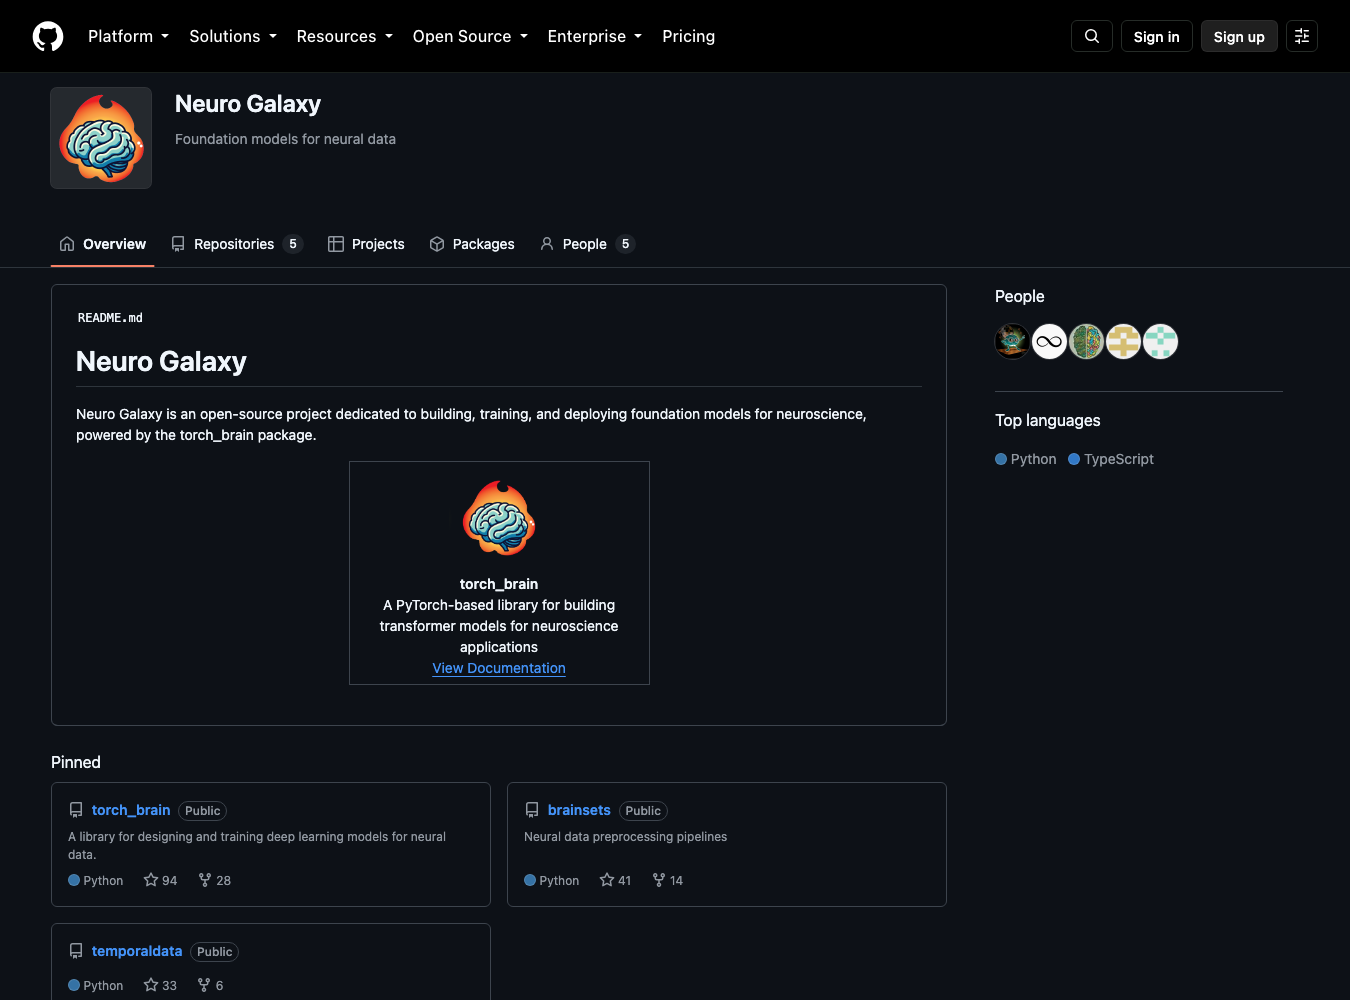
\includegraphics[width=\linewidth,height=43mm,keepaspectratio]{assets/history/neuro-galaxy-page.png}\par\smallskip
      {\tiny Neuro Galaxy / official GitHub organization\par}
  \end{columns}
  {\tiny\color{NTXMuted}Sources: \href{https://github.com/neuro-galaxy}{Neuro Galaxy}; \href{https://github.com/neuro-galaxy/torch_brain}{torch\_brain}; \href{https://nwb.org/events/hck26-2026-janelia-ndrh/}{ReHack 2026 program}\par}
  \note{[65:45--67:15] Neuro Galaxy provides an open-source framework, not one universal model or a commercial implant platform. The current torch\_brain repository says temporaldata and brainsets have been merged into it; pin versions when following older tutorials. Data loading supports neural and behavioral modalities, including spikes and regularly sampled signals. The verified event link is Alexandre Andre's July 14 Janelia tutorial. A separate NeuroGalaxy-branded hackathon has not yet been identified; do not invent its name, date or results. The proposed chapter project is Morgan's opportunity narrative, not an announced program. Retain classical baselines and held-out evaluation; access to code alone does not establish generalization or clinical readiness.}
\end{frame}
